\chapter{Random Variables}

\section{Introduction}
\begin{definition}[Discrete Random Variable]
    A discrete random variable assigns a discrete value to every outcome in the sample space \(\Omega\). 
\end{definition}

For example, we can assign the number of heads in tossing 3 coins to the random variable X. Then we have: 
\[
  \mathbb{P}(X = 0) = \dfrac{1}{8},\ \mathbb{P}(X = 1) = \dfrac{3}{8},\ \mathbb{P}(X = 2) = \dfrac{3}{8},\ \mathbb{P}(X = 3) = \dfrac{1}{8}.
\]

\subsection{Probability Mass Function (PMF)}
\begin{definition}[Probability Mass Function]
  The Probability Mass Function (PMF) \(p: \mathbb{R} \to [0, 1]\) of a discrete random variable \(X\) is the function 
  \[
    p_X(x) = \mathbb{P}(X = x)
  \]
\end{definition}

We can describe the PMF by a table:
\begin{table}[H]
    \centering
    \begin{tabular}{c|c|c|c|c}
        \(x\)  & 0 & 1 & 2 & 3  \\
      \midrule
        \(p_X(x)\)  & \(\frac{1}{8}\) & \(\frac{3}{8}\) & \(\frac{3}{8}\) & \(\frac{1}{8}\)  \\
    \end{tabular}
\end{table}

For every random variable \(X\), its probability mass function satisfies the following (based on the axioms of probability):

1. For every \(x \in \mathbb{R}, p(x) \geq 0\) is non-negative

2. If \(\mathcal{X}\) is the set of all possible values of \(X\), then the PMF values on \(\mathcal{X}\) will add up to 1:
\[
  \sum_{x \in X} p_X(x) = 1. 
\]

\begin{eg}
We roll two 3-sided dice. Let random variable \(D\) be the difference between the output of the first and second dice. What is the PMF of random variable \(D\)? What is the probability that \(D \geq 1\)?

\textbf{Solution:} 
For sample space, we have
\[
  \Omega = \{(1, 1), (1, 2), (1, 3), \cdots, (3, 3)\} \Longrightarrow D = x, x \in [-2, +2]
\]
\newpage

For PMF, we have:
\begin{table}[H]
  \centering
  \begin{tabular}{c|c|c|c|c|c}
      \(x\)  & \(-2\) & \(-1\) & \(0\) & \(1\) & \(2\)  \\
    \midrule
      \(p_X (x)\)  & \(\frac{1}{9}\) & \(\frac{2}{9}\) & \(\frac{3}{9}\) & \(\frac{2}{9}\) & \(\frac{1}{9}\)
  \end{tabular}
\end{table}

Then, for the probability that \(D \geq 1\), we have 
\[
  \mathbb{P}(D \geq 1) = p_X (1) + p_X (2) = \dfrac{2}{9} + \dfrac{1}{9} = \dfrac{3}{9}
\]
\end{eg}

\section{Bernoulli Random Variable}
\subsection{Definition}
A Bernoulli(\(p\)) random variable \(X\) shows the result of a trial where \(X = 1\) for the success outcome with probability \(p\) and \(X = 0\) for the failure outcome with probability \(1 - p\). 
\[
    X_i = \begin{dcases}
        1, &\text{ if Experiment \(i\) is succeeded }  ;\\
        0, &\text{ otherwise}  ;
    \end{dcases}
\]
with 
\[
  \begin{dcases}
    p_X (0) = 1 - p \\
    p_X (1) = p 
  \end{dcases}
\]

\subsection{PMF of Bernoulli Random Variable}
The probability mass function of a Bernoulli random variable can be easily found and comes in handy for some complicated calculations.  

For a Bernoulli random variable, we have an indicator random variable of an event \(A\), where \(I_A = 1\) if and only if \(A\) occurs.  

The PMF of a Bernoulli random variable is as follows:  
\[
  p_{I_A}(1) = \mathbb{P} (I_A = 1) = \mathbb{P} (A)
\]

\section{Discrete Uniform Random Variable}
A discrete uniform random variable takes values in a certain range, and each one of the values in that range has the same probability.  

Such a variable is determined by two parameters \(a, b\ (a \leq b)\), which define the beginning and the end of the range.  

Then, for every value of the random variable, the probability is \(\frac{1}{b - a + 1}\).  

We also need to consider one special case where \(a = b\). In this case, the random variable is deterministic, i.e., a constant value.

\section{Binomial Random Variable}
\subsection{Definition}
We call \(X\) a Binomial \((n, p)\) Random Variable when \(X\) represents the number of successes over \(n\) independent trials, each with a success probability of \(p\).

For example, if we toss \(n\) coins, the number of heads is Binomial\((n,\frac{1}{2})\) 

\begin{eg}
We flip a coin 10 times and consider the random variable of the number of consecutive changes (HT or TH) in the 10 coin flips. What is this random variable?

\textbf{Solution:} 
We have a total of 9 trials, with the possible outcomes being HH, HT, TH, and TT. The probability of a consecutive change is \(\frac{1}{2}\). This gives Binomial\((9, \frac{1}{2})\). 
\end{eg}

\begin{eg}
  We draw a 10-card hand from a 52-card deck. Let \(N =\) Number of Aces among the picked cards. What is the random variable \(N\)?
  
  \textbf{Solution:} 
  The definition states that the events must be independent. However, the second draw is influenced by the outcome of the first draw, so the events are not independent.
\end{eg}

\subsection{PMF of Binomial Random Variable}
The probability mass function (PMF) of a Binomial\((n, p)\) Random Variable is 
\[
  p_X (k) = \mathbb{P}(X = k) = \binom{n}{k}p^k(1 - p)^{n-k}
\]

\begin{minipage}{0.5\textwidth}
  \centering
  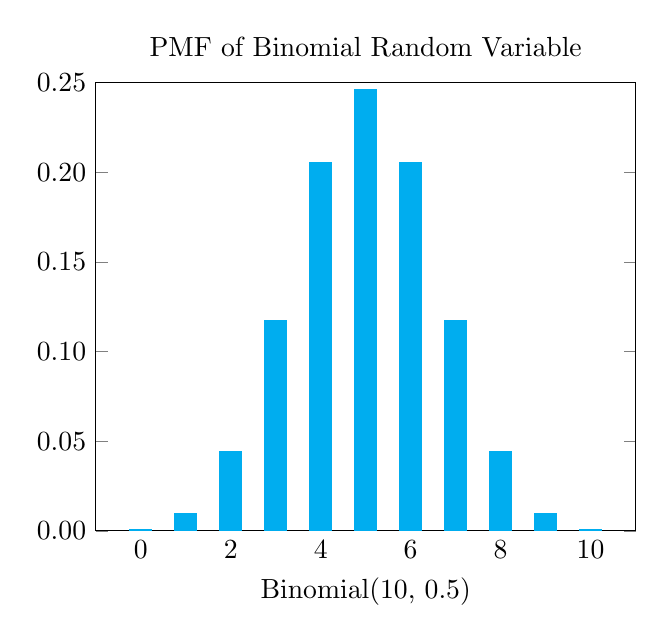
\begin{tikzpicture}
    \begin{axis}
    [
        % Define probability distribution functions
        declare function={
            binom(\n,\p) = \n!/(x!*(\n-x)!)*\p^x*(1-\p)^(\n-x);
            normal(\m,\s) = 1/(\s*sqrt(2*pi))*exp(-((x-\m)^2)/(2*\s^2));
        },
        % Plotting options
        title=PMF of Binomial Random Variable,
        ymin=0,
        ymax=0.25,
        xlabel={Binomial(10, 0.5)},
        samples at={0,...,10},
        xtick style={draw=none},
        yticklabel style={
            /pgf/number format/fixed,
            /pgf/number format/fixed zerofill,
            /pgf/number format/precision=2,
        },   
    ]
    
    % Plot Binomial Distribution
    \addplot [ybar=0pt,bar width=8pt,fill=cyan,draw=cyan] {binom(10,0.5)};
    \end{axis}
    \end{tikzpicture}
\end{minipage}
\begin{minipage}{0.5\textwidth}
  \centering
  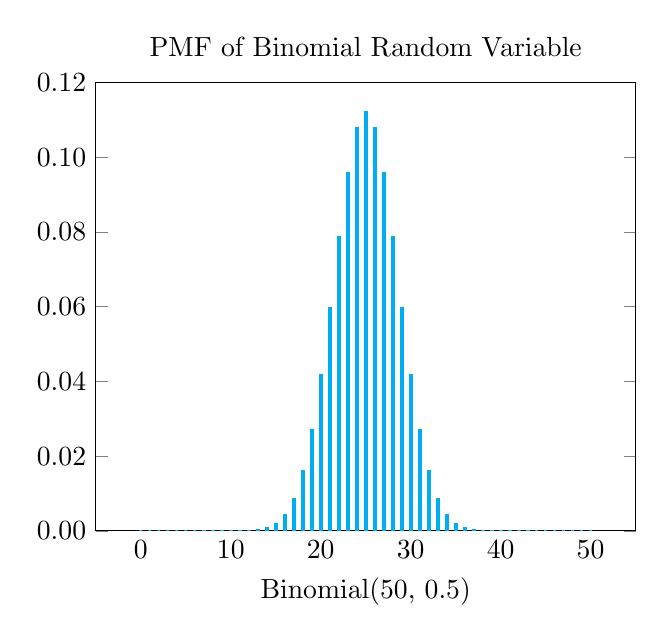
\begin{tikzpicture}
    \begin{axis}
    [
        % Define probability distribution functions
        declare function={
            binom(\n,\p) = \n!/(x!*(\n-x)!)*\p^x*(1-\p)^(\n-x);
            normal(\m,\s) = 1/(\s*sqrt(2*pi))*exp(-((x-\m)^2)/(2*\s^2));
        },
        % Plotting options
        title=PMF of Binomial Random Variable,
        ymin=0,
        ymax=0.12,
        xlabel={Binomial(50, 0.5)},
        samples at={0,...,50},
        xtick style={draw=none},
        yticklabel style={
            /pgf/number format/fixed,
            /pgf/number format/fixed zerofill,
            /pgf/number format/precision=2,
        },   
    ]
    
    % Plot Binomial Distribution
    \addplot [ybar=0pt,bar width=1pt,fill=cyan,draw=cyan] {binom(50,0.5)};
    \end{axis}
    \end{tikzpicture}
\end{minipage}

From the figures above, we can observe that as the value of \(n\) increases, the graph is symmetric around the central point. For  Binomial\((10, 0.5)\), the probability reaches its maximum at \(x = 5\), which can also be calculated as \(10 \times 0.5\). The same pattern holds for the graph on the right-hand side. This also makes sense because the probability of the event occurring is 0.5. Therefore, we can estimate that half of the events will occur, resulting in the maximum probability at \(x = 5\).

\begin{minipage}{0.5\textwidth}
  \centering
  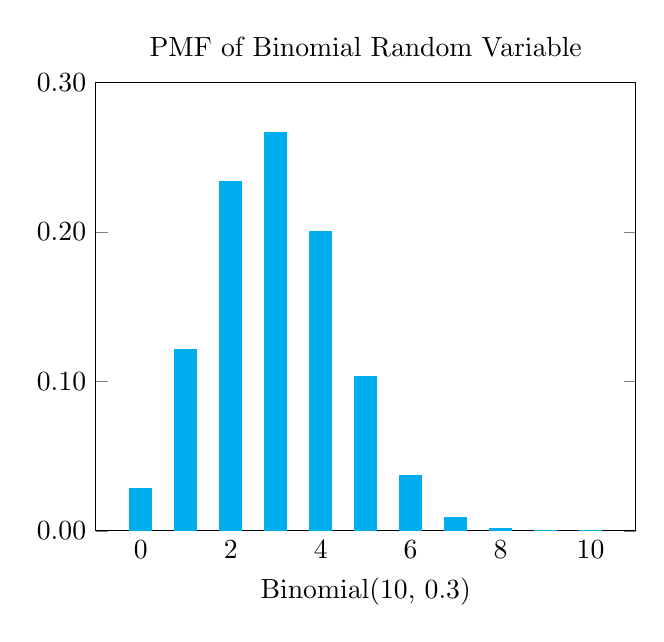
\begin{tikzpicture}
    \begin{axis}
    [
        % Define probability distribution functions
        declare function={
            binom(\n,\p) = \n!/(x!*(\n-x)!)*\p^x*(1-\p)^(\n-x);
            normal(\m,\s) = 1/(\s*sqrt(2*pi))*exp(-((x-\m)^2)/(2*\s^2));
        },
        % Plotting options
        title=PMF of Binomial Random Variable,
        ymin=0,
        ymax=0.3,
        xlabel={Binomial(10, 0.3)},
        samples at={0,...,10},
        xtick style={draw=none},
        yticklabel style={
            /pgf/number format/fixed,
            /pgf/number format/fixed zerofill,
            /pgf/number format/precision=2,
        },   
    ]
    
    % Plot Binomial Distribution
    \addplot [ybar=0pt,bar width=8pt,fill=cyan,draw=cyan] {binom(10,0.3)};
    \end{axis}
    \end{tikzpicture}
\end{minipage}
\begin{minipage}{0.5\textwidth}
  \centering
  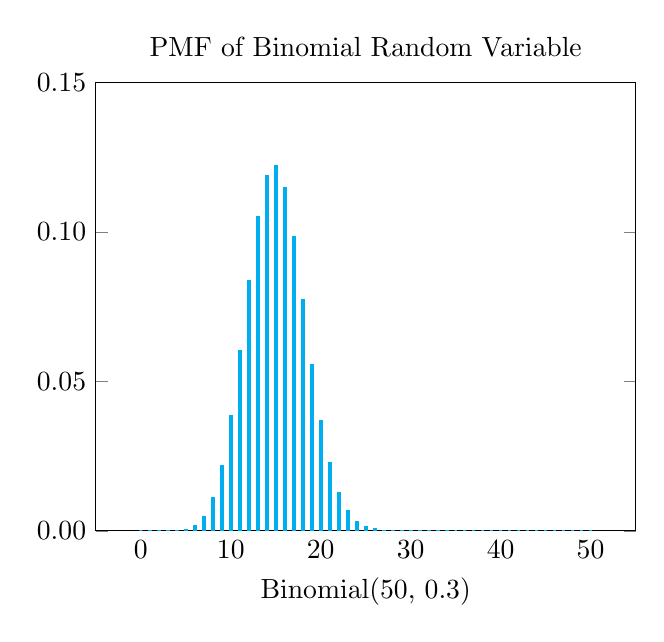
\begin{tikzpicture}
    \begin{axis}
    [
        % Define probability distribution functions
        declare function={
            binom(\n,\p) = \n!/(x!*(\n-x)!)*\p^x*(1-\p)^(\n-x);
            normal(\m,\s) = 1/(\s*sqrt(2*pi))*exp(-((x-\m)^2)/(2*\s^2));
        },
        % Plotting options
        title=PMF of Binomial Random Variable,
        ymin=0,
        ymax=0.15,
        xlabel={Binomial(50, 0.3)},
        samples at={0,...,50},
        xtick style={draw=none},
        yticklabel style={
            /pgf/number format/fixed,
            /pgf/number format/fixed zerofill,
            /pgf/number format/precision=2,
        },   
    ]
    
    % Plot Binomial Distribution
    \addplot [ybar=0pt,bar width=1pt,fill=cyan,draw=cyan] {binom(50,0.3)};
    \end{axis}
    \end{tikzpicture}
\end{minipage}

For the two graphs above, it also holds true that the maximum value is reached at \(10 \times 0.3 = 3\) or \(50 \times 0.3 = 15\), due to the same reasoning. However, in this case, the graph is no longer symmetric around the central point.

Additionally, we observe that the graph shifts to the left when \(p < 0.5\). Conversely, if \(p > 0.5\), the graph shifts to the right.

\begin{eg}
The Lakers and the Celtics meet for a 7-game playoff. 

Lakers win 60\% of the time. What is the probability that all 7 games are played? What is the probability that Lakers win the play-off in 6 games? 

\textbf{Solution:} 
For all 7 games to be played, the first 6 games must occur, which means that both the Lakers and the Celtics win 3 games each. So \(X\) is a Binomial\((6, 0.6)\). 
\[
  \mathbb{P}(X = 3) = \binom{6}{3} \times (0.6)^3 \times (1 - 0.6)^3 = \dfrac{864}{3125}
\]

For the Lakers to win in 6 games, we cannot simply use \(\mathbb{P}(X = 4)\) because it also includes the probability of the Lakers winning in 4 or 5 games. However, by fixing the Lakers to win the 6th game, we can define a new variable following Binomial\((5, 0.6)\). We then only need to calculate the probability of the Lakers winning 3 games in the first 5 games.
\[
  \mathbb{P}(X = 3) \times 0.6 = \binom{5}{3} \times (0.6)^3 \times (1 - 0.6)^2 \times 0.6 = \dfrac{648}{3125}
\]
\end{eg}

\section{Geometric Random Variable}
\subsection{Definition}
We call \(N\) a Geometric\((p)\) Random Variable when \(X\) represents the first time of success over a series of independent trials \(X_1, X_2, \cdots\), each with a success probability of \(p\):
\[
  N = \text{first (smallest)}\ n\ \text{such that}\ X_n = 1.
\]

For example, we toss a coin until we see the first heads. The number of coin tosses to see the first heads is Geometric(\(\frac{1}{2}\)). 

\subsection{PMF of Geometric Random Variable}
The probability mass function (PMF) of a Geometric\((p)\) Random Variable is 
\[
  p_X (k) = \mathbb{P}(X = k) = p(1 - p)^{k-1} 
\]

Axioms of probability also holds for PMF of geometric random variable. Therefore, 
\[
  \sum_{k = 1}^{\infty} p(1 - p)^{k-1} = 1  
\]

\begin{minipage}{0.5\textwidth}
  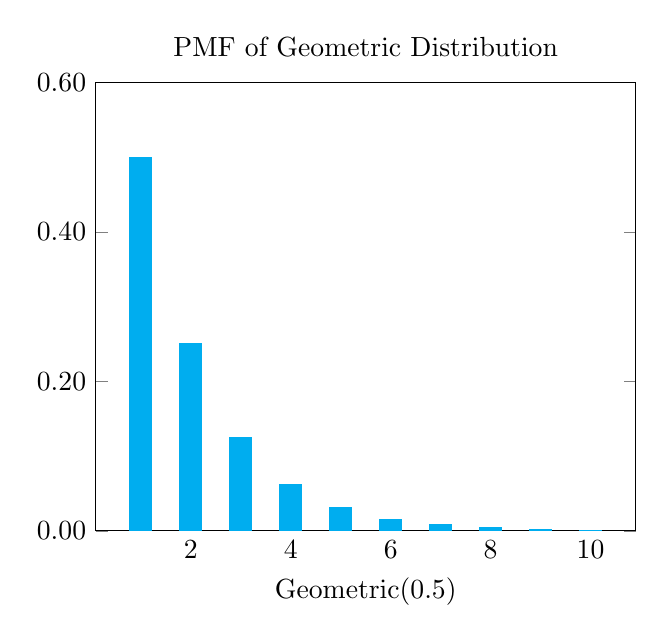
\begin{tikzpicture}
    \begin{axis}[
        title = {PMF of Geometric Distribution},
        ymin=0,
        ymax=0.6,
        xlabel = {Geometric(0.5)},
        samples at={1,...,10},
        xtick style={draw=none},
          yticklabel style={
              /pgf/number format/fixed,
              /pgf/number format/fixed zerofill,
              /pgf/number format/precision=2,
        },   
        domain=1:10,
        samples=10,
    ]
    % Define p, probability of success
    \pgfmathsetmacro{\p}{0.5}
    
    % Plot the PMF of the geometric distribution
    \addplot [
      ybar=0pt,
      bar width=8pt,
      fill=cyan,
      draw=cyan,
      mark=none,
  ] {(\p*(1-\p)^(x-1))};
    \end{axis}
    \end{tikzpicture}
\end{minipage}
\begin{minipage}{0.5\textwidth}
  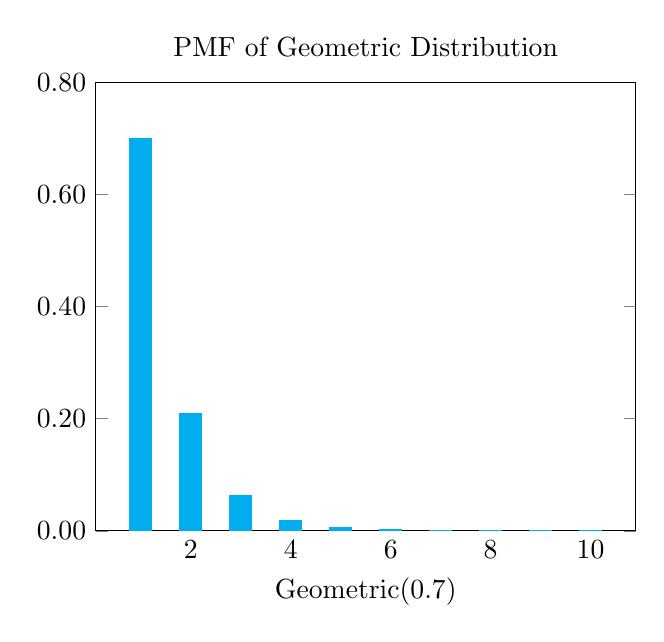
\begin{tikzpicture}
    \begin{axis}[
        title = {PMF of Geometric Distribution},
        ymin=0,
        ymax=0.8,
        xlabel = {Geometric(0.7)},
        samples at={1,...,10},
        xtick style={draw=none},
          yticklabel style={
              /pgf/number format/fixed,
              /pgf/number format/fixed zerofill,
              /pgf/number format/precision=2,
        },   
        domain=1:10,
        samples=10,
    ]
    % Define p, probability of success
    \pgfmathsetmacro{\p}{0.7}
    
    % Plot the PMF of the geometric distribution
    \addplot [
      ybar=0pt,
      bar width=8pt,
      fill=cyan,
      draw=cyan,
      mark=none,
  ] {(\p*(1-\p)^(x-1))};
    \end{axis}
    \end{tikzpicture}
\end{minipage}

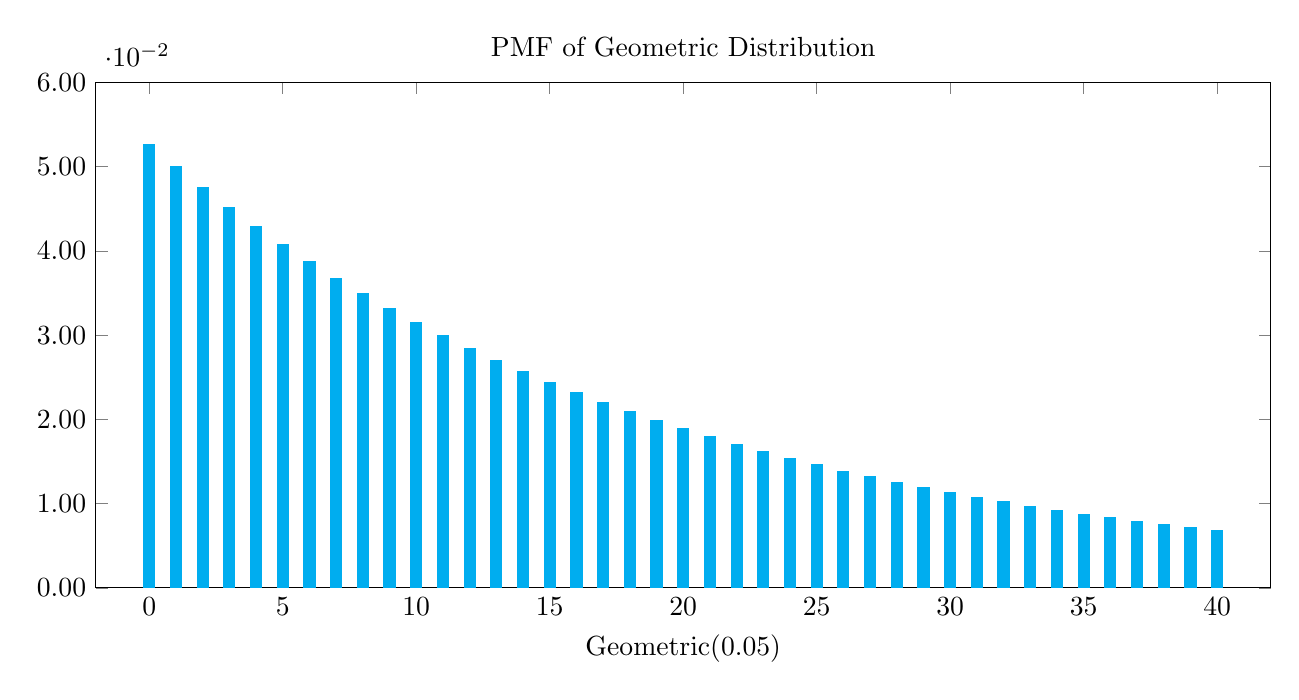
\begin{tikzpicture}
    \begin{axis}[
        title = {PMF of Geometric Distribution},
        ymin=0,
        ymax=0.06,
        xmin=-2,
        xmax=42,
        xlabel = {Geometric(0.05)},
        samples at={0,...,40},
        xtick={0,5,...,40},
        height=8cm,
        width=16.5cm,
          yticklabel style={
              /pgf/number format/fixed,
              /pgf/number format/fixed zerofill,
              /pgf/number format/precision=2,
        },   
        domain=1:40,
        samples=40,
    ]
    % Define p, probability of success
    \pgfmathsetmacro{\p}{0.05}
    
    % Plot the PMF of the geometric distribution
    \addplot [
      ybar=0pt,
      bar width=4pt,
      fill=cyan,
      draw=cyan,
      mark=none,
  ] {(\p*(1-\p)^(x-1))};
    \end{axis}
\end{tikzpicture}

\begin{eg}
You keep rolling dice until you roll a 6. What is the probability that you rolled more than 10 times? 

\textbf{Solution:} 
Define \(X\) is a Geometric(\(\frac{1}{6}\)), then we have 
\[ 
  \mathbb{P}(X \geq 11) = \sum_{k = 11}^{\infty} p(1 - p)^{k-1} = \sum_{k = 11}^{\infty} \dfrac{1}{6} \times (\dfrac{5}{6})^{k-1} = \left(\dfrac{5}{6}\right)^{10}
\]
\end{eg}

By generalizing the above, we have 
\[
  \sum_{k = m}^{\infty} p(1 - p)^{k-1} = (1 - p)^{m-1}   
\]
This formula means that if we want to find the probability of success occurring at or after the \(m\)-th trial, we can treat the trials before the \(m\)-th one as all failures. This simplifies the calculation.

\section{Cumulative Distribution Function (CDF)}
\begin{definition}[Cumulative Distribution Function (CDF)]
  For a random variable \(X\), its cumulative distribution function (CDF) \(F(x)\) is:
  \[
    F(x) = \mathbb{P}(X \leq x)
  \]
\end{definition}

From the definition of PMF, we have 
\[
  F(x) = \sum_{\substack{k \in \mathcal{X} \\ k \leq x}} p(x) 
\]

For a Geometric(\(p\)) random variable \(X\), the CDF will be 
\[
  F(k) = \mathbb{P}(X \leq k) = 1 - \mathbb{P}(X > k) = 1- (1 - p)^k
\]

For a Binomial(\(n, p\)) random variable \(X\), the CDF will be 
\[
  F(k) = \mathbb{P}(X \leq k) = (1 - p)^n + n(1 - p)^{n-1}p + \cdots + \binom{n}{k} (1 - p)^{n-k} p^k
\]

\begin{eg}
You keep rolling dice until you roll a 6. What is the probability that you roll the dice an even number of times?

\textbf{Solution 1:} 
\[
\begin{aligned}
  \mathbb{P}(X \text{is even}) &= \mathbb{P}(X = 2) + \mathbb{P}(X = 4) + \mathbb{P}(X = 6) + \cdots \\
  &= p(2) + p(4) + p(6) + \cdots \\
  &= \dfrac{1}{6} \times \dfrac{5}{6} + \dfrac{1}{6} \times \left(\dfrac{5}{6}\right)^3 + \dfrac{1}{6} \times \left(\dfrac{5}{6}\right)^5 + \cdots
\end{aligned}
\]

\textbf{Solution 2:}
Let's define event \(A\) as the event that an even number is rolled. Next, we define another event \(B\), which is independent of event \(A\), such that using conditional probability, we have \(\mathbb{P}(A) = \mathbb{P}(A \vert B)\). 

For example, we can define \(B = \{X = 1\ \text{or}\ X = 2\}\). Since \(A\) and \(B\) are independent, we can then proceed with the calculation.
\[
  \mathbb{P}(A \vert B) = \dfrac{\mathbb{P}(A \cap B)}{\mathbb{P}(B)} = \dfrac{\mathbb{P}(X = 2)}{\mathbb{P}(X = 1) + \mathbb{P}(X = 2)} = \dfrac{p(1 - p)}{p + p(1 - p)} = \dfrac{p - 1}{p - 2} = \dfrac{\frac{5}{6}}{\frac{11}{6}} = \dfrac{5}{11}
\]
\end{eg}

\newpage
\section{Poisson Random Variable}
\begin{eg}
  Alice randomly sprinkles 25 chocolate chips on 5 cookies.
  
  1. What is the random variable \(N\) on how many chips a cookie gets?
  \[
    N \sim\ \text{Binomial}(25, \frac{1}{5})
  \]
  2. What is the probability a cookie gets no chips?
  \[
    \mathbb{P}(N = 0) = \binom{25}{0} \times (\dfrac{1}{5})^0 \times (1 - \dfrac{1}{5})^{25} = 0.004
  \]
  3. What is the probability a cookie gets exactly 5 chips?
  \[
    \mathbb{P}(N = 5) = \binom{25}{5} \times (\dfrac{1}{5})^5 \times (1 - \dfrac{1}{5})^{20} = 0.196
  \]
  4. What is the probability a cookie gets at most 5 chips?
  \[
    \mathbb{P}(N \leq 5) \approx 0.617
  \]
\end{eg}

We now want to examine how the probability changes if we increase the values, for example, by having 250 chocolate chips and 50 cookies instead. Intuitively, the probability should not change significantly, and through calculation, the results are indeed similar to those obtained in the previous example. 

\begin{minipage}{0.5\textwidth}
  \centering
  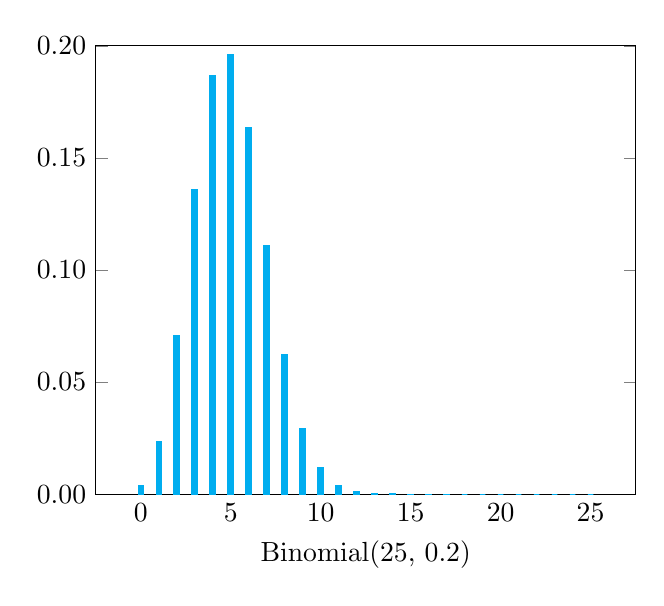
\begin{tikzpicture}
    \begin{axis}
    [
        % Define probability distribution functions
        declare function={
            binom(\n,\p) = \n!/(x!*(\n-x)!)*\p^x*(1-\p)^(\n-x);
            normal(\m,\s) = 1/(\s*sqrt(2*pi))*exp(-((x-\m)^2)/(2*\s^2));
        },
        % Plotting options
        ymin=0,
        ymax=0.2,
        xlabel={Binomial(25, 0.2)},
        samples at={0,...,25},
        xtick style={draw=none},
        yticklabel style={
            /pgf/number format/fixed,
            /pgf/number format/fixed zerofill,
            /pgf/number format/precision=2,
        },   
    ]
    
    % Plot Binomial Distribution
    \addplot [ybar=0pt,bar width=2pt,fill=cyan,draw=cyan] {binom(25,0.2)};
    \end{axis}
    \end{tikzpicture}
\end{minipage}
\begin{minipage}{0.5\textwidth}
  \centering
  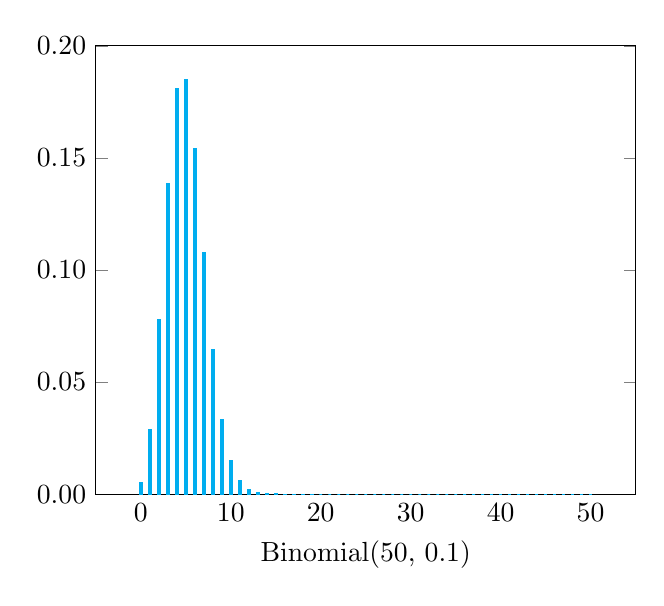
\begin{tikzpicture}
    \begin{axis}
    [
        % Define probability distribution functions
        declare function={
            binom(\n,\p) = \n!/(x!*(\n-x)!)*\p^x*(1-\p)^(\n-x);
            normal(\m,\s) = 1/(\s*sqrt(2*pi))*exp(-((x-\m)^2)/(2*\s^2));
        },
        % Plotting options
        ymin=0,
        ymax=0.2,
        xlabel={Binomial(50, 0.1)},
        samples at={0,...,50},
        xtick style={draw=none},
        yticklabel style={
            /pgf/number format/fixed,
            /pgf/number format/fixed zerofill,
            /pgf/number format/precision=2,
        },   
    ]
    
    % Plot Binomial Distribution
    \addplot [ybar=0pt,bar width=1pt,fill=cyan,draw=cyan] {binom(50,0.1)};
    \end{axis}
    \end{tikzpicture}
\end{minipage}

From the above, we see that when we double the value, the PMF remains quite similar to the previous one. Additionally, the average rate of chocolate chips per cookie is also the same, i.e., \(25 \times 0.2 = 50 \times 0.1 = 5\). 

\begin{table}[H]
  \centering
  \begin{tabular}{c|c|c|c}
      \toprule
      Poisson(5) & \(\mathbb{P}(X = 0)\) & \(\mathbb{P}(X = 5)\) & \(\mathbb{P}(X \leq 5)\)  \\
    \midrule
      Binomial(\(25, 0.2\)) & 0.004 & 0.196 & 0.617  \\
      Binomial(\(50, 0.1\)) & 0.005 & 0.185 & 0.616  \\
      Binomial(\(500, 0.01\)) & 0.006 & 0.176 & 0.615  \\
      \bottomrule
  \end{tabular}
\end{table}

From the values above, we can see that the probability converges to a certain value. This is what we call a Poisson Random Variable. The values we obtain by using \(25 \times 0.2, 50 \times 0.1\) represent the rate of Poisson random variable.

\begin{definition}[Poisson Random Variable]
  A Poisson(\(\lambda\)) random variable \(X\) has the PMF:
  \[
    p(k) = e^{-\lambda}\dfrac{\lambda^k}{k!}, \quad k = 0, 1, 2, 3, \cdots, \text{where \(\lambda\) is called the rate parameter.}
  \]
\end{definition}

\begin{theorem}
  Poisson(\(\lambda\)) is the limit approximation of Binomial(\(n, \frac{\lambda}{n}\)) when \(n \to \infty\): 
  \[
    \mathbb{P}(\text{Poisson}(\lambda) = k) = \lim_{n \to \infty} \mathbb{P}(\text{Binomial}(n, \dfrac{\lambda}{n}) = k)
  \]
\end{theorem}

Poisson random variable can be used when we have a large number of independent trials while the expected number of successes remains small (the rate of successes being constant). 

\begin{eg}
  Suppose rain is falling on your head a rate of 3 drops/sec. What is the probability that you get 
  
  (1) no hits in the next second? 
  
  \textbf{Solution:} 
  \[
    \mathbb{P}(\text{Poisson}(3) = 0) = e^{-3}\dfrac{3^0}{0!} = e^{-3} \approx 0.050
  \]

  (2) at least 3 hits in the next second? 

  \textbf{Solution:} 
  \[
    \mathbb{P}(\text{Poisson}(3) \geq 3) = 1 - \mathbb{P}(\text{Poisson}(3) < 3) = 1 - e^{-3}\dfrac{3^0}{0!} - e^{-3}\dfrac{3^1}{1!} - e^{-3}\dfrac{3^2}{2!} = 1 - \dfrac{17}{2 e^{3}} \approx 0.576
  \]

  (3) exactly 10 hits in the next 5 seconds?

  \textbf{Solution:} 
  \[
    \mathbb{P}(\text{Poisson}(3 \times 5) = 10) = e^{-15}\dfrac{15^{10} }{10!} = 0.049
  \]
\end{eg}

\section{Properties of Random Variables}

\subsection{Expected Value}
\begin{definition}[Expected Value]
  The expected value (expectation) of a random variable \(X\) with PMF \(p(x)\) is 
  \[
    \mathbb{E}[X] = \sum_{x} xp_X (x)
  \]
\end{definition}

For example, the expected value of random variable \(X\) as the number of heads in tossing 1 coin:
\[
  \mathbb{E}[X] = \dfrac{1}{2} \times 0 + \dfrac{1}{2} \times 1 = \dfrac{1}{2}
\]
Now, instead of flipping one coins, we flip 3 coins. For PMF, we have 
\[
  p(k) = \binom{3}{k} (\dfrac{1}{2})^k (\dfrac{1}{2})^{3-k} = \dfrac{\binom{3}{k}}{8}
\]
Then, the expected value of random variable \(X\) as the number of heads in tossing 3 coin:
\[
  \mathbb{E}[X] = \dfrac{1}{8} \times 0 + \dfrac{3}{8} \times 1 + \dfrac{3}{8} \times 2 + \dfrac{1}{8} \times 3 = \dfrac{3}{2}
\]

The expectation is the average value the random variable takes when the experiment is done many times.

\begin{eg}
  Find the expected value of random variable F as the face value of a six-sided die. 

  \textbf{Solution:} 
  \[
    \mathbb{E}[X] = 1 \times \dfrac{1}{6} + 2 \times \dfrac{1}{6} + 3 \times \dfrac{1}{6} + 4 \times \dfrac{1}{6} + 5 \times \dfrac{1}{6} + 6 \times \dfrac{1}{6} = \dfrac{7}{2}
  \]
\end{eg}

\begin{eg}
  We play this game that we roll three dice, and you win \(k\) dollars if we see \(k \geq 1\) "Two" outcomes. You lose 1 dollar if we see no "Two" outcomes.

  Should you play this game?

  \textbf{Solution:}
  \[
    G = -1, \mathbb{P}(-1) = (\dfrac{5}{6})^3 = \dfrac{125}{216};\quad G = 1, \mathbb{P}(1) = \binom{3}{1}(\dfrac{1}{6})(\dfrac{5}{6})^2 = \dfrac{25}{72};
  \]
  \[
    G = 2, \mathbb{P}(2) = \binom{3}{2}(\dfrac{1}{6})^2(\dfrac{5}{6})^1 = \dfrac{5}{72};\quad G = 3, \mathbb{P}(3) = (\dfrac{1}{6})^3 = \dfrac{1}{216};
  \]
  \[
    \mathbb{E}[X] = -1 \times \dfrac{125}{216} + 1 \times \dfrac{25}{72} + 2 \times \dfrac{5}{72} + 3 \times \dfrac{1}{216} = - \dfrac{17}{216} \approx -0.079
  \]
  Therefore, it’s better not to play this game. 
\end{eg}

\subsection{Function of Random Variables}
If \(X\) is a random variable with PMF \(p_X\), then \(Y = f(X)\) will also be a random variable with PMF \(p_Y\):
\[
  p_Y(y) = \sum_{x: f(x)=y} p_X(x)
\]

The expected value of \(f(X)\) for a function \(f\) and random variable \(X\) is 
\[
  \mathbb{E}[f(X)] = \sum_{x} f(x)p_X(x) 
\]

\begin{eg}
Consider a random variable \(X\) with the following PMF: 
\begin{center}
\begin{tabular}{c|c|c|c}
      \toprule
      \(x\)  & 0 & 1 & 2  \\
    \midrule
      \(p(x)\)  & \(\frac{1}{3}\) & \(\frac{1}{3}\) & \(\frac{1}{3}\)  \\
      \bottomrule
  \end{tabular}
  \quad\quad
  \begin{tabular}{c|c|c|c}
      \toprule
      \(y = X - 1\)  & \(-1\)  & 0 & 1  \\
    \midrule
      \(p(y)\)  & \(\frac{1}{3}\) & \(\frac{1}{3}\) & \(\frac{1}{3}\)  \\
      \bottomrule
\end{tabular}
\quad\quad
\begin{tabular}{c|c|c}
  \toprule
  \(z = (X - 1)^2\)  & 0 & 1  \\
\midrule
  \(p(z)\)  & \(\frac{1}{3}\) & \(\frac{2}{3}\)  \\
  \bottomrule
\end{tabular}
\end{center}

Using \(Y = (X - 1)^2\) as an example, we have: 
\[
  p_Y(1) = \sum_{x: (x - 1)^2=1} p_X(x) = p_X(0) + p_X(2) = \dfrac{2}{3}
\]

Additionally, for the expected values of the above PMF, we have: 
\[
\begin{aligned}
  \mathbb{E}[X] &= 0 \times \dfrac{1}{3} + 1 \times \dfrac{1}{3} + 2 \times \dfrac{1}{3} = 1 \\
  \mathbb{E}[X - 1] &= -1 \times \dfrac{1}{3} + 0 \times \dfrac{1}{3} + 1 \times \dfrac{1}{3} = 0 \\
  \mathbb{E}[(X - 1)^2] &= 0 \times \dfrac{1}{3} + 1 \times \dfrac{2}{3} = \dfrac{2}{3} \\
\end{aligned}
\]

Alternatively, we can use the following method to directly calculate the expected values:
\[
\begin{aligned}
  \mathbb{E}[X - 1] &= \sum_{x \in \{0, 1, 2\}}(x - 1)p(x) = (0 - 1) \times \dfrac{1}{3} + (1 - 1) \times \dfrac{1}{3} + (2 - 1) \times \dfrac{1}{3} = 0 \\
  \mathbb{E}[(X - 1)^2] &= \sum_{x \in \{0, 1, 2\}}(x - 1)^2 p(x) = (0 - 1)^2 \times \dfrac{1}{3} + (1 - 1)^2 \times \dfrac{1}{3} + (2 - 1)^2 \times \dfrac{1}{3} = \dfrac{2}{3}
\end{aligned}
\]

\end{eg}

\begin{remark}
  \[
    \mathbb{E}[f(x)] \neq f(\mathbb{E}[X])
  \]
\end{remark}
\begin{eg}
  Suppose the distance between place A and place B is 1 km. There is a 60\% chance that the weather will be sunny; in that case, you will walk from A to B at a speed of 5 km/h. Conversely, there is a 40\% chance that the weather will be rainy; in that case, you will take a shuttle traveling at a speed of 30 km/h. Find the expected value of time \(T\) and speed \(V\).

  \textbf{Solution:} 
  Given that \(V = \frac{1}{T}\),
  \[
    \mathbb{E}[V] = 0.6 \times 5 + 0.4 \times 30 = 15\ \text{km/h}
  \]
  \[
    \mathbb{E}[T] = \mathbb{E}[\frac{1}{V}] = 0.6 \times \frac{1}{5} + 0.4 \times \frac{1}{30} = \frac{2}{15}\ \text{h} \neq \dfrac{1}{\mathbb{E}[V]}
  \]
\end{eg}

% END OF DOCUMENT